% =====================================================================
%  Mid-Semester Project Presentation (title + 10 slides)
%   1 Introduction/Motivation (1)          | 2-3 Literature survey (2)
%   4 Objectives + specs, 5 Block diagram  (Objectives/Block/Spec: 2)
%   6-8 Work carried out, results, discussion (3)
%   9 Timeline (1)                          | 10 References (1)
%  Compile with pdflatex (Overleaf). Fill in [[ ... ]] placeholders.
% =====================================================================
\documentclass[aspectratio=169,10pt]{beamer}
\usetheme{Madrid}
\setbeamertemplate{navigation symbols}{}
\usepackage{booktabs}
\usepackage{amsmath,amssymb}
\usepackage{tikz}
\usetikzlibrary{positioning,arrows.meta}
\graphicspath{{figures/}}

\title[AnatoPhaseNet]{AnatoPhaseNet: Subject-Independent Pathological Gait
Classification from Silhouettes}
\author[Project Group]{[[Student Name 1]] \and [[Student Name 2]]\\[1mm]
\small Supervisor: [[Supervisor Name]]}
\institute{[[Department]], [[Institute]]}
\date{Mid-Semester Project Evaluation}

\tikzset{
  b/.style={draw, rounded corners=2pt, align=center, font=\scriptsize,
            minimum height=9mm, text width=19mm, fill=blue!6},
  n/.style={b, fill=orange!15},
  a/.style={b, fill=red!10},
  o/.style={b, fill=green!12},
  arr/.style={-{Stealth[length=1.6mm]}, thick}}

\begin{document}

\begin{frame}
\titlepage
\end{frame}

% ---------------------------------------------------------------- 1
\begin{frame}{Introduction and Motivation}
\begin{itemize}
\item Parkinson's, diplegia, hemiplegia and neuropathy each leave a
characteristic walking pattern.
\item A \textbf{single side-view camera + silhouette} is cheap and
privacy-preserving, unlike a marker-based gait lab.
\item Published silhouette models report \textbf{$>$99\,\%} (CRA-Net: 99.16\,\%
on GAIT-IT), but with the \emph{same people} in training and test.
\item A diagnostic tool always sees a \textbf{new patient}.
\end{itemize}
\begin{block}{Aim}
A biomechanically motivated model, evaluated only on \textbf{unseen subjects}
(10-fold subject-exclusive cross-validation).
\end{block}
\end{frame}

% ---------------------------------------------------------------- 2
\begin{frame}{Literature Survey (1/2): Gait Pathology Classification}
\small
\begin{tabular}{@{}p{3.4cm}p{6.0cm}p{4.0cm}@{}}
\toprule
Work & Idea & Limitation \\
\midrule
Verlekar \textit{et al.} 2018 & GEI + transfer-learned CNN & one static image per walk \\
Loureiro \& Correia 2020 & skeleton energy image & static summary \\
Albuquerque \textit{et al.} 2021 & GAIT-IT dataset, subject-independent protocol & hand-crafted pipeline \\
SE / CBAM / Non-local & channel / spatial attention & generic, frame-level \\
\textbf{CRA-Net} (Bodepu \textit{et al.}) & encoder--decoder + reverse cross-attention fusion, 0.93\,M & frames independent; subjects shared \\
\bottomrule
\end{tabular}
\end{frame}

% ---------------------------------------------------------------- 3
\begin{frame}{Literature Survey (2/2): Video and Gait Modelling}
\begin{itemize}
\item \textbf{(2+1)D convolution} (Tran 2018): spatial $1{\times}3{\times}3$ +
temporal $3{\times}1{\times}1$.
\item \textbf{TSM} (Lin 2019): temporal mixing with zero extra parameters.
\item \textbf{SSAN} (Guo 2021): separable spatial / temporal self-attention.
\item \textbf{GaitSet} (Chao 2019): horizontal body-strip pooling.
\item \textbf{Gradient reversal} (Ganin 2015): adversarial removal of a nuisance
factor.
\end{itemize}
\begin{alertblock}{Gap}
No model combines gait-phase alignment, body-part temporal features and posture
geometry, and near-perfect results are not measured on unseen subjects.
\end{alertblock}
\end{frame}

% ---------------------------------------------------------------- 4
\begin{frame}{Objectives and Target Specifications}
\begin{columns}[T]
\column{0.44\textwidth}
\textbf{Objectives}
\begin{enumerate}\small
\item Classify a gait cycle of an \emph{unseen} subject (5 GAIT-IT classes,
INIT classes).
\item Walk-level diagnosis from all cycles.
\item Severity: normal / mild / severe.
\item Run on a 4\,GB laptop GPU.
\end{enumerate}
\column{0.54\textwidth}
\small
\begin{tabular}{@{}lll@{}}
\toprule
Spec (GAIT-IT) & Target & Achieved \\
\midrule
Cycle accuracy & $\geq95\,\%$ & \textbf{95.47\,\%} \\
Macro-F1 & $\geq0.95$ & \textbf{0.962} \\
Walk accuracy & $\geq96\,\%$ & \textbf{96.28\,\%} \\
Worst fold & $\geq90\,\%$ & 87.4\,\% \\
Severity & $\geq80\,\%$ & 80.68\,\% \\
Parameters & $\leq6$\,M & 5.00\,M \\
Input & $9{\times}96^2$ & $9{\times}96^2$ \\
GPU & 4\,GB & RTX 3050 \\
\bottomrule
\end{tabular}
\end{columns}
\end{frame}

% ---------------------------------------------------------------- 5
\begin{frame}{Block Diagrams: Initial vs.\ Final Architecture}
\textbf{Initial: ST-CRANet} (6.59\,M params, 12 uniform frames, $128^2$)\\[1mm]
\centering
\resizebox{0.95\textwidth}{!}{%
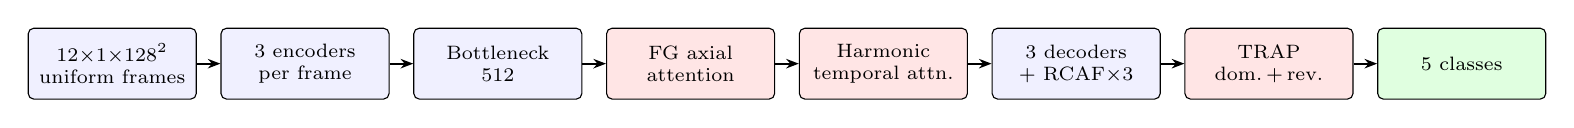
\begin{tikzpicture}[node distance=3mm]
\node[b] (in) {$12{\times}1{\times}128^2$\\uniform frames};
\node[b, right=of in] (enc) {3 encoders\\per frame};
\node[b, right=of enc] (bot) {Bottleneck\\512};
\node[a, right=of bot] (ax) {FG axial\\attention};
\node[a, right=of ax] (hp) {Harmonic\\temporal attn.};
\node[b, right=of hp] (dec) {3 decoders\\+ RCAF$\times$3};
\node[a, right=of dec] (trap) {TRAP\\dom.\,+\,rev.};
\node[o, right=of trap] (fc) {5 classes};
\draw[arr] (in)--(enc); \draw[arr] (enc)--(bot); \draw[arr] (bot)--(ax);
\draw[arr] (ax)--(hp); \draw[arr] (hp)--(dec); \draw[arr] (dec)--(trap);
\draw[arr] (trap)--(fc);
\end{tikzpicture}}
\\[3mm]
\raggedright\textbf{Final: AnatoPhaseNet v6} (5.00\,M params, 9 clinical phases, $96^2$)\\[1mm]
\centering
\resizebox{0.95\textwidth}{!}{%
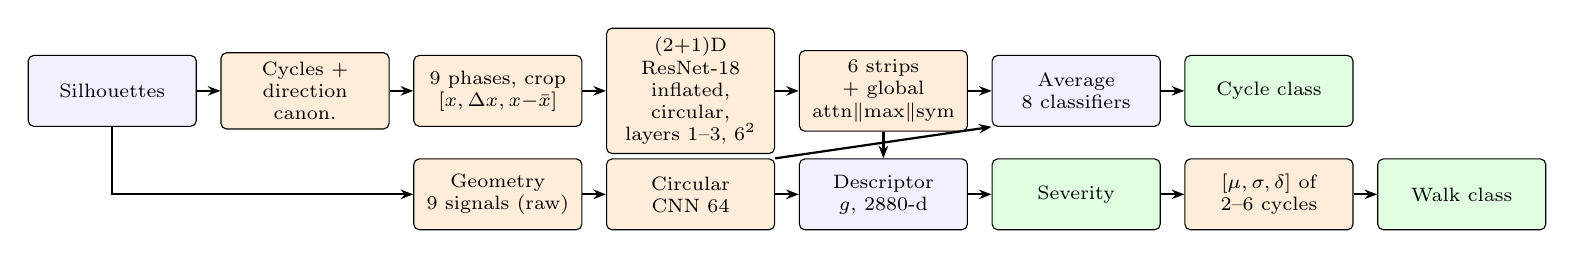
\begin{tikzpicture}[node distance=3mm and 3mm]
\node[b] (sil) {Silhouettes};
\node[n, right=of sil] (cyc) {Cycles +\\direction canon.};
\node[n, right=of cyc] (ph) {9 phases, crop\\$[x,\Delta x,x{-}\bar x]$};
\node[n, right=of ph] (bb) {(2+1)D ResNet-18\\inflated, circular,\\layers 1--3, $6^2$};
\node[n, right=of bb] (pt) {6 strips + global\\attn$\Vert$max$\Vert$sym};
\node[b, right=of pt] (avg) {Average\\8 classifiers};
\node[o, right=of avg] (o1) {Cycle class};
\node[n, below=4mm of ph] (geo) {Geometry\\9 signals (raw)};
\node[n, right=of geo] (gc) {Circular\\CNN 64};
\node[b, right=of gc] (g) {Descriptor\\$g$, 2880-d};
\node[o, right=of g] (sev) {Severity};
\node[n, right=of sev] (mc) {$[\mu,\sigma,\delta]$ of\\2--6 cycles};
\node[o, right=of mc] (o2) {Walk class};
\draw[arr] (sil)--(cyc); \draw[arr] (cyc)--(ph); \draw[arr] (ph)--(bb);
\draw[arr] (bb)--(pt); \draw[arr] (pt)--(avg); \draw[arr] (avg)--(o1);
\draw[arr] (sil.south) |- (geo.west); \draw[arr] (geo)--(gc);
\draw[arr] (gc.north east) -- (avg.south west);
\draw[arr] (gc)--(g); \draw[arr] (pt.south) -- (g.north);
\draw[arr] (g)--(sev); \draw[arr] (sev)--(mc); \draw[arr] (mc)--(o2);
\end{tikzpicture}}
\\[1mm]
\scriptsize Red: added to CRA-Net in the initial model. Orange: introduced in the final model.
\end{frame}

% ---------------------------------------------------------------- 6
\begin{frame}{Work Carried Out (1/3): What Changed and Why}
\scriptsize
\begin{tabular}{@{}p{2.6cm}p{5.4cm}p{5.0cm}l@{}}
\toprule
Change & Why (problem found) & Key formula / proof & Cycle acc. \\
\midrule
0. Subject-exclusive folds & random split shared subjects (ST-CRANet: 100\,\% train, 77.24\,\% val) & $\mathcal S_i\cap\mathcal S_j=\emptyset$ & -- \\
1. 9 clinical phases & uniform frame $i$ has phase $\phi_i=(i\frac{L-1}{T-1}\bmod P)/P$, different in every walk & $x_\alpha(\tau_p/\alpha)=x(\tau_p)$: speed-invariant; 828$\rightarrow$3813 samples & 89.10 \\
2. Regions, $96^2$ crop, focal loss & limbs only $\sim$35\,px & magnify $H/h_{\text{box}}$; $\mathcal L=-\sum(1-p_c)^{1.5}\tilde y_c\log p_c$ & 93.01 \\
3a. Direction canon. & back walk $\approx$ mirror of front (corr.\ 0.65$\rightarrow$0.996) & flip asymmetry encoded direction, not limbs & \\
3b. Full inflation & only 1 conv/stage pretrained, no BN & BN$_t$: $\gamma{=}0\Rightarrow\mathbf v{=}\mathrm{ReLU}(\mathbf u){=}\mathbf u$: exact ResNet-18 at start & \\
3c. Circular temporal conv & cycle is periodic; zero pad adds edges & $W\circledast S_r\mathbf u=S_r(W\circledast\mathbf u)$ & \\
3d. 6 strips + half-cycle sym. & $3{\times}3$ map; legs alternate in \emph{time} & $\mathbf s=\frac14\sum_{t=0}^{3}|\mathbf f_t-\mathbf f_{t+4}|$ & \\
3e. Part-classifier ensemble & 3\,M-param head, $\sim$17 subjects & $\mathrm{Var}(\bar z)=\sigma^2(\rho+\frac{1-\rho}{P})\le\sigma^2$ & 94.05 \\
\bottomrule
\end{tabular}
\end{frame}

% ---------------------------------------------------------------- 7
\begin{frame}{Work Carried Out (2/3): v5 and v6 Additions}
\small
\begin{itemize}
\item \textbf{Severity multi-task} (labels \texttt{lvl1}/\texttt{lvl2}):
severity 35.96\,\% $\rightarrow$ \textbf{79.59\,\%}, cycle accuracy unchanged
(94.76 vs.\ 94.81).
\item \textbf{Stride variability}: walk from $K=2$--6 cycles,
$\ \boldsymbol\mu,\ \boldsymbol\sigma=\sqrt{\tfrac{1}{K-1}\sum(\mathbf e_k-\boldsymbol\mu)^2},\
\boldsymbol\delta=\tfrac1{K-1}\sum|\mathbf e_{k+1}-\mathbf e_k|$.
Walk accuracy 94.57 $\rightarrow$ \textbf{95.71\,\%}.
\item \textbf{Geometry branch.} \emph{Proof that cropping loses height:} crop
$R_t$ scales by $H/h_t$, so output height is $H$ for every $h_t$, and crouch,
stoop and bob become invisible. Remedy: 9 raw signals, normalised by the
walk's median height, $s h_t/(s\tilde h)=h_t/\tilde h$ (scale-invariant).
Cycle accuracy \textbf{95.47\,\%}, diplegic recall 84.0 $\rightarrow$
\textbf{87.9\,\%}.
\item \textbf{Subject adversary} (gradient reversal,
$\lambda=0.1(\frac{2}{1+e^{-10p}}-1)$): 95.16\,\%, no gain, so it stays off.
\end{itemize}
\vspace{1mm}
\scriptsize Loss: $\mathcal L=\mathcal L_{\text{FL}}(\bar z)+0.5\mathcal
L_{\text{part}}+0.3\mathcal L_{\text{sev}}+1.0\mathcal L_{\text{walk}}$; AdamW
$10^{-3}$, 20 epochs, EMA 0.98, 3-view TTA, $\sqrt{n_c}$ class balance (6.2:1
$\rightarrow$ 2.5:1).
\end{frame}

% ---------------------------------------------------------------- 8
\begin{frame}{Work Carried Out (3/3): Results and Discussion}
\begin{columns}[T]
\column{0.56\textwidth}
\scriptsize
\begin{tabular}{@{}lccc@{}}
\toprule
GAIT-IT, 10-fold & Cycle (\%) & F1 & Walk (\%) \\
\midrule
ST-CRANet$^\dagger$ & 77.24 & 0.788 & -- \\
ST-PhaseNet & $89.10\pm4.56$ & 0.901 & 92.72 \\
v3 & $93.01\pm5.38$ & 0.937 & 94.54 \\
v4 & $94.05\pm4.04$ & 0.949 & 94.57 \\
v5 & $94.81\pm4.63$ & 0.955 & 95.71 \\
\textbf{v6} & $\mathbf{95.47\pm4.11}$ & \textbf{0.962} & \textbf{96.28} \\
\bottomrule
\end{tabular}\\
$^\dagger$random split (val.); others subject-exclusive.\\[2mm]
\begin{itemize}
\item Recall: normal 100, neurop.\ 99.7, hemipl.\ 96.8, Parkins.\ 96.5,
diplegic 87.9.
\item Main error: diplegic $\leftrightarrow$ Parkinsonian (both bilateral,
flexed).
\item Folds 3 and 9 weakest in every version, so the errors are
subject-specific.
\item INIT-6: $93.27\pm4.71\,\%$ (v5); INIT-8: 85.56\,\% (v4).
\end{itemize}
\column{0.42\textwidth}
\centering
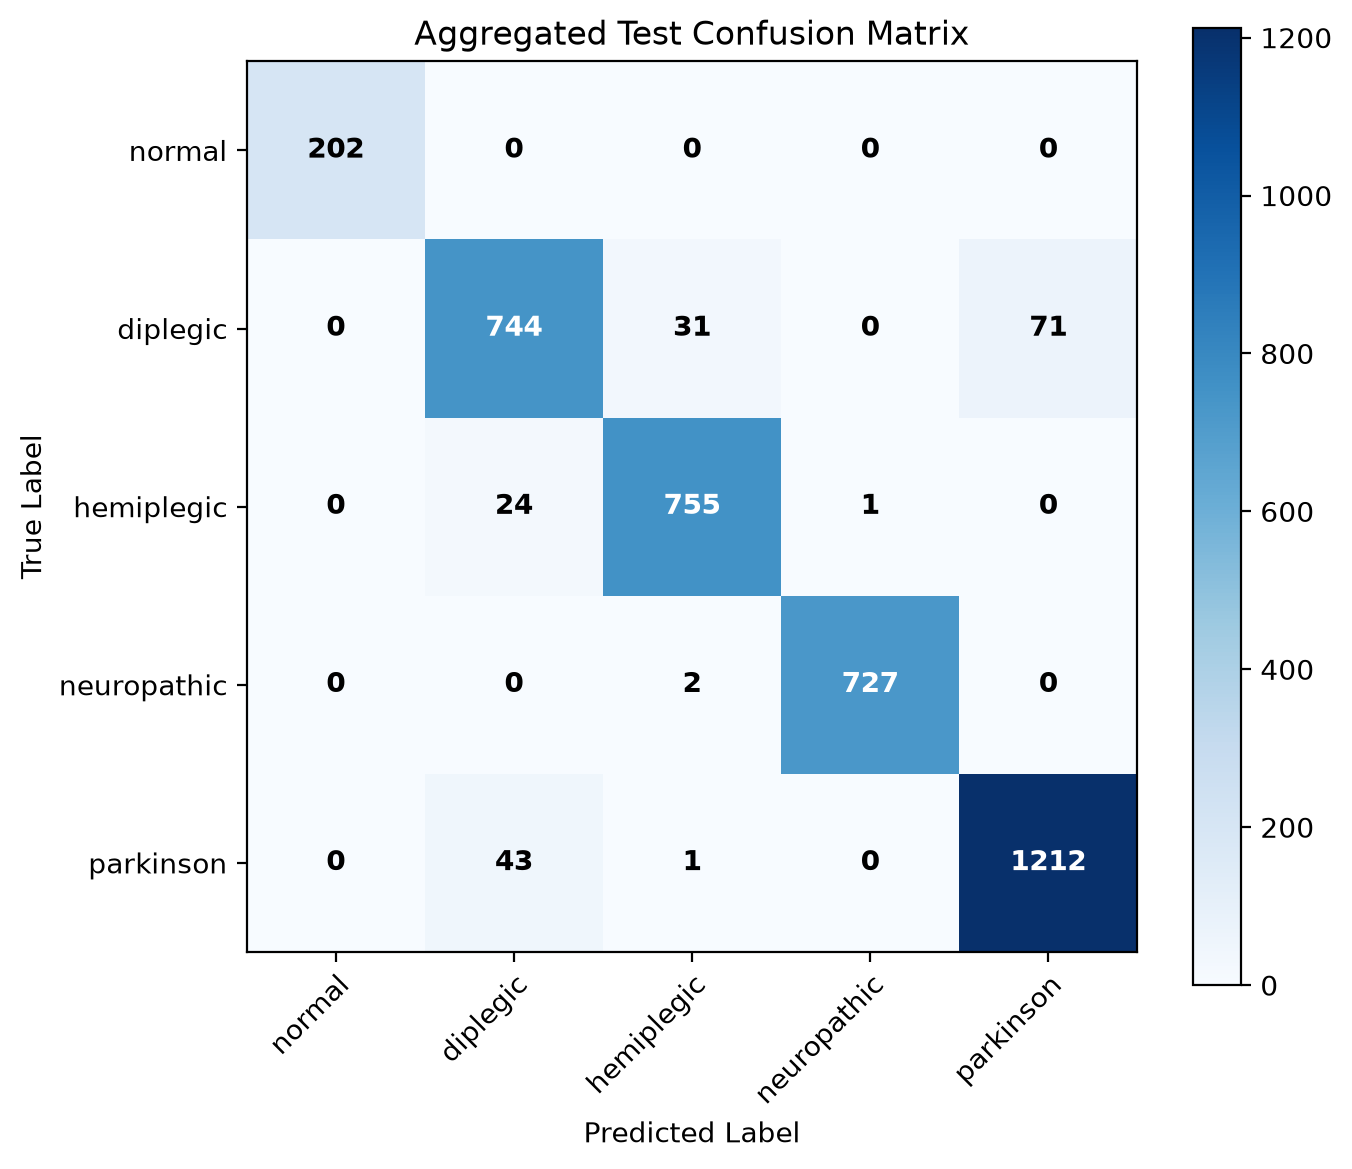
\includegraphics[width=\linewidth]{cm_gaitit_v6.png}
\end{columns}
\end{frame}

% ---------------------------------------------------------------- 9
\begin{frame}{Timeline}
\small
\begin{tabular}{@{}lp{8.4cm}l@{}}
\toprule
Stage & Work & Result \\
\midrule
1 & Literature survey, datasets, ST-CRANet & 77.24\,\% (leaky) \\
2 & Subject-exclusive protocol, ST-PhaseNet & 89.10\,\% \\
3 & AnatoPhaseNet v1--v3 & 93.34\,\% best \\
4 & v4 redesign, INIT support & 94.05\,\% \\
5 & v5 severity + stride variability & 94.81\,\% \\
6 & v6 geometry branch, subject adversary & \textbf{95.47\,\%} \\
\midrule
\emph{Next} & \emph{v6 on INIT; multi-seed runs; per-change ablations} & \\
\emph{Next} & \emph{weak folds 3/9; diplegic vs.\ Parkinsonian; saliency maps} & \\
\emph{Final} & \emph{cross-dataset test; final report; paper} & \\
\bottomrule
\end{tabular}
\end{frame}

% ---------------------------------------------------------------- 10
\begin{frame}{References}
\tiny
\begin{thebibliography}{9}
\bibitem{a} P. Albuquerque \textit{et al.}, ``Remote gait type classification
system using markerless 2D video,'' \emph{Diagnostics}, vol.~11, no.~10,
p.~1824, 2021.
\bibitem{b} J. Ortells, M.~T. Herrero-Ezquerro, and R.~A. Mollineda,
``Vision-based gait impairment analysis for aided diagnosis,'' \emph{Med. Biol.
Eng. Comput.}, vol.~56, pp.~1553--1564, 2018.
\bibitem{c} D. Bodepu, M.~I. Junaid, S. Madarapu, J.~P. Sahoo, and S. Ari,
``CRA-Net: Cross reverse attention network for classification of
neuro-degenerative diseases based on gait analysis,'' \emph{Biomed. Signal
Process. Control}.
\bibitem{d} T.~T. Verlekar, P.~L. Correia, and L.~D. Soares, ``Using transfer
learning for classification of gait pathologies,'' in \emph{Proc. IEEE BIBM},
2018.
\bibitem{e} J. Loureiro and P.~L. Correia, ``Using a skeleton gait energy image
for pathological gait classification,'' in \emph{Proc. IEEE FG}, 2020.
\bibitem{f} D. Tran \textit{et al.}, ``A closer look at spatiotemporal
convolutions for action recognition,'' in \emph{Proc. IEEE CVPR}, 2018.
\bibitem{g} J. Lin, C. Gan, and S. Han, ``TSM: Temporal shift module for
efficient video understanding,'' in \emph{Proc. IEEE ICCV}, 2019.
\bibitem{h} X. Guo, X. Guo, and Y. Lu, ``SSAN: Separable self-attention network
for video representation learning,'' in \emph{Proc. IEEE CVPR}, 2021.
\bibitem{i} H. Chao, Y. He, J. Zhang, and J. Feng, ``GaitSet: Regarding gait as
a set for cross-view gait recognition,'' in \emph{Proc. AAAI}, 2019.
\bibitem{j} K. He, X. Zhang, S. Ren, and J. Sun, ``Deep residual learning for
image recognition,'' in \emph{Proc. IEEE CVPR}, 2016.
\bibitem{k} Y. Ganin and V. Lempitsky, ``Unsupervised domain adaptation by
backpropagation,'' in \emph{Proc. ICML}, 2015.
\end{thebibliography}
\end{frame}

\end{document}
